%
% This work may be distributed and/or modified under the
% conditions of the LaTeX Project Public License, either version 1.3
% of this license or (at your option) any later version.
% 
% The Current Maintainer of this work is P. S. Eduardo.
%
% This work consists of the file poli.cls.
%% -----------------------------------------------------------------
% Escola Politécnica UFRJ LaTeX Template
% Version: 2303
% Author: Filipe Santos Pacheco Prates
% email: filipespprates@gmail.com
% Base: CoppeTeX 2.3
%%------------------------------------------------------------------
\documentclass[grad,pdftex]{poli}
\usepackage[utf8]{inputenc}
\usepackage{amsmath,amssymb}
\usepackage{float}
\usepackage{multirow}
\usepackage{longtable}
\usepackage{tikz}
\usepackage{listings}
\definecolor{codegreen}{rgb}{0,0.6,0}
\definecolor{codegray}{rgb}{0.5,0.5,0.5}
\definecolor{codepurple}{rgb}{0.58,0,0.82}
\definecolor{backcolour}{rgb}{0.95,0.95,0.92}


\lstdefinelanguage{JavaScript}{
  keywords={typeof, new, true, false, catch, function, return, null, catch, switch, var, if, in, while, do, else, case, break},
  keywordstyle=\color{blue}\bfseries,
  ndkeywords={class, export, boolean, throw, implements, import, this},
  ndkeywordstyle=\color{darkgray}\bfseries,
  identifierstyle=\color{black},
  sensitive=false,
  comment=[l]{//},
  morecomment=[s]{/*}{*/},
  commentstyle=\color{purple}\ttfamily,
  stringstyle=\color{red}\ttfamily,
  morestring=[b]',
  morestring=[b]"
}

\lstset{
   language=JavaScript,
   backgroundcolor=\color{lightgray},
   extendedchars=true,
   basicstyle=\footnotesize\ttfamily,
   showstringspaces=false,
   showspaces=false,
   numbers=left,
   numberstyle=\footnotesize,
   numbersep=9pt,
   tabsize=2,
   breaklines=true,
   showtabs=false,
   captionpos=b
}


\usetikzlibrary{shapes,arrows,chains,positioning}
\usepackage{enumitem}
\usepackage{indentfirst}
\usepackage{array}
\usepackage{diagbox}
\usepackage{natbib}
%\usepackage[alf, bibjustif]{abntex2cite}

\makelosymbols
\makeloabbreviations

\begin{document}
  \title{@placeholder TCC do prates}
  \foreigntitle{@placeholder TCC do prates}
  \author{Filipe}{S. P. Prates}
  \advisor{Prof.}{Daniel}{R. Figueiredo}{Ph.D.}
  %\coadvisor{Prof.}{Nome}{Sobrenome}{D.Sc.}
  \examiner{Prof.}{Nome Completo}{Ph.D.}
  \examiner{Prof.}{Nome Completo}{D.Sc.}
  %\examiner{Prof.}{Nome Completo}{D.Sc.}
  \department{ECI} %UTTILIZE A SIGLA DO SEU DEPARTAMENTO MODIFICAR OS NOMES DE CURSO, DEPARTAMENTO E OBTENÇÃO DE GRAU (Obs: caso tenha algum equívoco nesses argumentos, necessário modificar o arquivo poli.cls no local que faz a leitura deste argumento)
  \date{2}{2023}
  \keyword{keyword1}
  \keyword{keyword2}
  \keyword{keyword3}
  \keyword{keyword4}
  \maketitle

  \frontmatter
  \dedication{``@placeholder'' - Autor desconhecido.}


  \chapter*{Agradecimentos}

Agradeça seus pais, seus professores, seus amigos e eu acreditando que ninguém fosse ler esse capítulo, mas no meu TCC teve professor corrigindo texto aqui rsrsr.
  \begin{abstract}

% Descrição de uma aplicação web intuitiva para gerenciamento de dados em um banco de dados em grafo. \\ \\
% (Cliente:Vue.js-Nuxt.js-ApolloClient)←[:GRAPHQL]→(Servidor:Node.js-ApolloServer-@neo4j/graphql)←[:CYPHER]→(Banco de Dados: Neo4j)
\end{abstract}


  \begin{foreignabstract}

@placeholder english abstract

\end{foreignabstract}


  \tableofcontents
  \listoffigures
  \listoftables
  \printlosymbols
  \printloabbreviations

  \mainmatter
    \chapter{Introdução}

\section{Motivação}

Gerenciar os dados armazenados em um banco de dados é fundamental para qualquer sistema de informação. Tal gerenciamento precisa ser eficiente, rápido e intuitivo, de maneira à evitar alterações equivocadas e garantir que os usuários do sistema interajam com dados atualizados e corretos.

Para isso existem sistemas de gerenciamento de bancos de dados, com formulários dependendo da estrutura de tabelas e dados definidos no banco, e possibilidade de interagir com os dados através de uma linguagem de DCL (Data Control Language / Linguagem de Controle de Dados), soluções como phpMyAdmin, SQL Server Management Studio, ou o Oracle RDBMS trazem essas funcionalidades, porém exclusivamente para bancos de dados SQL.

Assumindo um banco de dados em grafo, em especial Neo4j Database, as ferramentas de gerenciamento de dados disponíveis se limitam à interações diretas por DCL (Neo4j Browser). Tal limitação gera abertura para alterações equivocadas nos dados e não permitem uma fácil visualização e gerenciamento intuitivo dos dados, especialmente quando utilizados por usuários ingênuos ao schema.

Foi então desenvolvido uma interface de gerenciamento de dados para bancos de dados Neo4j, através de uma API em Graphql, com foco na visualização, navegação e gerenciamento intuitivo dos dados do grafo armazenado. A interface recebe o schema do banco de dados e gera um ambiente de "Perfis e Listas", que permite a criação e edição de nós, seus relacionamentos, e os dados de cada um destes. Hoje o sistema é usado amplamente por mais de 30 colaboradores principalmente dos times de Qualidade, Desenvolvimento, Suporte e Educacional da empresa para qual foi desenvolvido.

\section{Contribuição}

Nesse trabalho documento o funcionamento e a arquitetura do sistema, tanto a interface do usuário, que é gerada através de componentes reutilizáveis e as ferramentas Nuxt.js, Vue.js e Apollo Client, como a camada intermediária que conecta a interface ao banco de dados, sendo utilizado o Node.js, Express.js, e a biblioteca oficial do Neo4j que conecta o banco de dados à uma API em GraphQL, @neo4j/graphql.

A interface do usuário segue uma dinâmica de navegação diferente, foi mapeado o isomorfismo de um nó e seus vizinhos com uma página de perfil, suas abas e seus elementos, de maneira que conseguimos gerar uma página de perfil para cada um dos nós no banco e facilmente ir navegando através de suas relações para os perfis de outros nós - alterando ou acrescentando dados arbitrariamente no processo.

\section{Organização}

Primeiro vamos ver as outras opções de gerenciamento de dados para bancos de dados Neo4j, explicitando a falta de uma solução como a proposta no trabalho. Após esses estudo, veremos um resumo de cada uma das principais ferramentas e tecnologias utilizadas no desenvolvimento do sistema. Então uma descrição da arquitetura do sistema e como foi desenvolvido, finalizando com a descrição de como o sistema é utilizado em produção.
    \chapter{Trabalhos Relacionados}
\label{chap2}

\section{Lorem Ipsum}
    
    \chapter{Tecnologias Utilizadas}
\label{chap3}

\section{GraphQL}

dadada


\section{Neo4j}
O Neo4j é um sistema de gerenciamento de banco de dados orientado a grafos desenvolvido pela Neo4j Inc., que opera sob uma estrutura de dados que consiste em nós, relacionamentos e propriedades. Ao contrário dos bancos de dados relacionais, que usam tabelas e linhas, o Neo4j permite que as informações sejam armazenadas em um formato altamente conectado, imitando as interações do mundo real. Isso faz do Neo4j uma escolha ideal para cenários onde as relações entre os dados são tão importantes quanto os próprios dados.

 
Cada Nó e cada Aresta possui um ou mais Rótulos (\textit{labels}), que definem o \textit{tipo} do dado e instanciam um index de lookup, funcionando similar à uma tabela num banco SQL. Podemos eficientemente recuperar os dados de todos os nós ou todas as arestas de um certo rótulo para listá-las, por exemplo.

Cada rótulo possui sua definição de \textit{tipo}, que define a tipagem de cada uma de suas propriedades, incluindo possíveis ligações com nós de mesmo, ou outro, rótulo.

\subsection{Cypher Query Language}

O banco Neo4j, diferentemente da maioria dos bancos relacionais, não utiliza SQL como a linguagem de manipulação de registros de dados, e sim a própria linguagem chamada Cypher.

\begin{figure}[H]
    \centering
    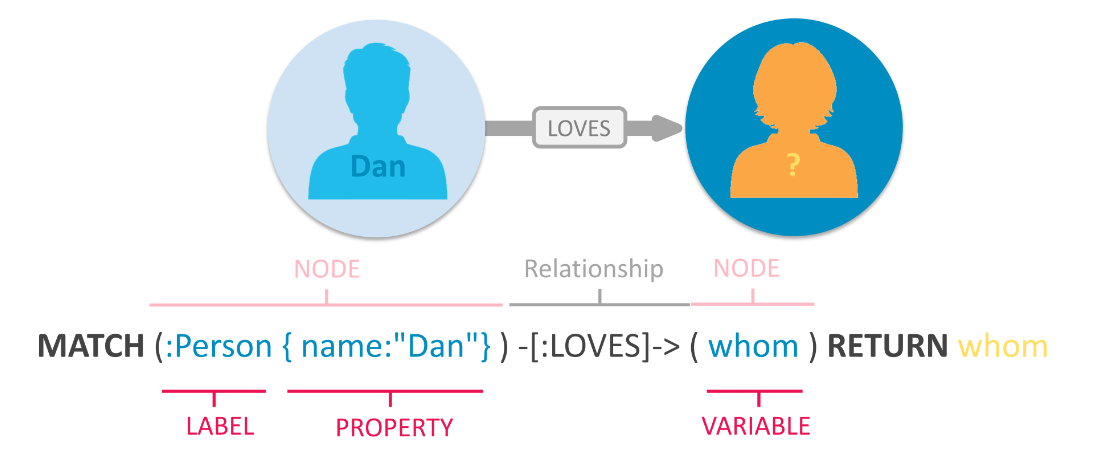
\includegraphics[width=1.0\linewidth]{Imagens/chap03/cypher-exemple.png}
    \caption{Exemplo Cypher https://neo4j.com/developer/cypher/.}
    \label{fig:profile-exemple}
\end{figure}
https://neo4j.com/developer/cypher/


\subsection{@neo4j/graphql}
A GraphQL to Cypher query execution layer for Neo4j and JavaScript GraphQL implementations.

Para realizar a conexão entre as requisições em GraphQL que a interface do usuário irá realizar com o banco de dados, precisamos realizar essa tradução para a Cypher Query Language que será executada no banco. Para tal trabalho a neo4j disponibiliza uma biblioteca que permite tanto definir e gerar o schema do banco de dados, como gerar automaticamente requisições de CRUD para cada um dos \textit{tipos} definidos.

Cada rótulo possui sua definição de \textit{tipo}, que define a tipagem de cada uma de suas propriedades, incluindo possíveis ligações com nós de mesmo, ou outro, rótulo.

\section{Apollo}

Biblioteca de gerenciamento de estados para Javascript, através de GraphQL. É composta pois duas partes que se comunicam entre si:
\begin{itemize}
    \item Apollo Client -> Utilizado na aplicação cliente. Permite funcionalidade de controle de requisição de dados, variáveis de carregamento, controle de cache, e variáveis de estados locais. Realizam requisições em GraphQL para:
    \item Apollo Server -> Servidor GraphQL compatível com qualquer cliente que envia uma requisição GraphQL a ele, incluindo Apollo Clients. Utilizado na geração do schema que as requisições (e consequentemente os dados) precisam seguir. É conectado com poder de gerenciamento à qualquer fonte de dados (no caso do sistema "Admins", um banco Neo4j).

\end{itemize}

\section{Node.js}

Software de código aberto baseado no interpretador V8 que permite a execução de códigos JavaScript em múltiplas plataformas.

\section{Express.js}

Framework web mais popular para node.js. Minimalista,  disponibilizando apenas funcionalidades básicas para desenvolvimento web como handling para diferentes verbos HTTP, e, crucialmente para o projeto, middlewares para camadas de autenticação e autorização.


\begin{lstlisting}
const express = require("express");
const app = express();
const port = 3000;

app.get("/", function (req, res) {
  res.send("Hello World!");
});

app.use(function (req, res, next) {
    if (!isRequestAllowed(req)) {
        return res.status(403).send({
            message: "You don't have permissions to execute this request.",
        });
    }
    return next();
});

app.listen(port, function () {
  console.log(`Porta de escuta: ${port}!`);
});
\end{lstlisting}


\section{Vue.js}

fala do v-model
    \chapter{Descrição do Sistema ``Admins''}
\label{chap4}

Dado a escolha de um banco de dados em grafo como o Neo4j, enfrentamos o problema de ser complicado para pessoas ingênuas ao schema do banco de dados manipularem os itens de dados, além de ser pouco seguro gerenciá-los diretamente através de uma Cypher.Desta forma é possível facilmente realizar consultas muito pesadas, ou que tem consequências difíceis de reverter, de maneira acidental.

O sistema ``Admins'' foi desenvolvido com o objetivo de proporcionar uma interface amigável para mais facilmente gerenciar os dados, evitando os problemas mencionados acima. Através desse sistema os usuários podem criar, editar, conectar e desconectar arbitrariamente qualquer nó no grafo do banco de dados. Esse sistema foi nomeado de ``Admins'', devido ao subdomínio utilizado para hospedá-lo (admins.jovensgenios.com).

\section{Perfis e Listas}

Junto com o time de Design, identificamos uma maneira de entender e visualizar o grafo que está armazenado no banco, dando para cada nó uma página de perfil, que mostra e permite edição de suas propriedades e relações, além de uma página de lista/pesquisa para cada rótulo (relevante) no banco de dados. Endentendo este isomorfismo, conseguimos criar esta interface e permitir os usuários navegarem e editarem o grafo de maneira intuitiva.

\begin{figure}[H]
    \centering
    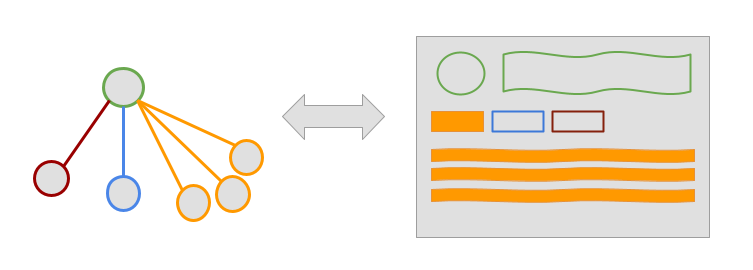
\includegraphics[width=1.0\linewidth]{Imagens/chap04/perfil-isomorfismo.png}
    \caption{Abstração de um \textbf{nó} (verde) está relacionado à \textbf{um nó de rótulo X} (vermelho), \textbf{um de rótulo Y} (azul), e possui relação com \textbf{três nós de rótulos Z} (amarelos) no grafo armazenado no banco de dados.}
    \label{fig:isomorphism}
\end{figure}

Temos então dois tipos de telas:
\begin{itemize}
    \item Perfis - Com as propriedades do nó na parte superior da tela, e diferentes abas (uma para cada tipo de relação que o nó dono possui) na parte inferior, sendo que dentro de cada aba, uma lista de elementos com os nós vizinhos através daquele tipo de relação. Tal lista possui hiperlinks para páginas de perfis deste vizinhos. Assim conseguimos andar pelo grafo através dos nós e relações, e em cada nó do caminho temos ações específicas como edição, criação ou conexão de nós.
        
    \begin{figure}[H]
        \centering
        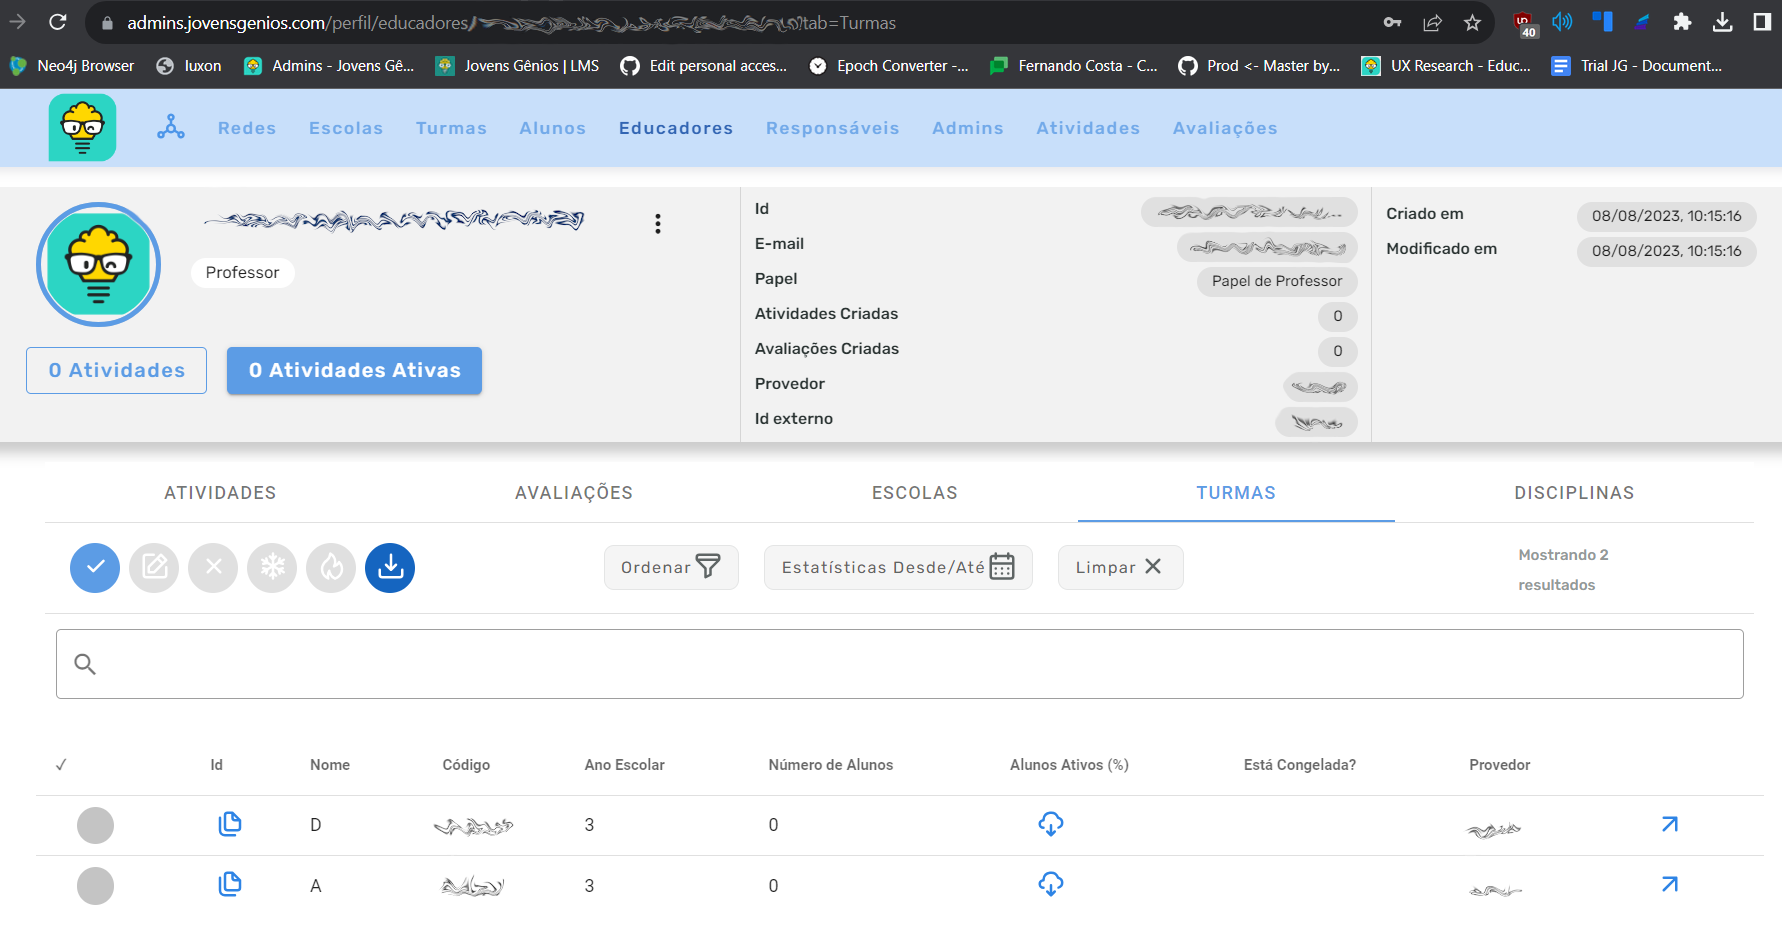
\includegraphics[width=1.0\linewidth]{Imagens/chap04/perfil-exemplo.png}
        \caption{Página de Perfil de um educador. Note as ações em azul ou cinza (dependente de selecionar um elemento para acessá-la) no cabeçalho da lista de vizinhos. Inclui edição, remoção e criação da aresta, entre o nó do perfil e os elementos selecionados, assim como outras ações específicas do \textit{tipo} da aba (Congelar/Descongelar turma).}
        \label{fig:profile-exemple}
    \end{figure}
    
    \item Listas - Precisamos começar a navegar pelo grafo a partir de algum nó inicial. Para isso existem as páginas de listas. Nelas são listados todos os elementos de um certo \textit{tipo} (de forma paginada), com hiperlinks para suas páginas de perfil. Também possui funcionalidades de busca e filtragem genéricas, além de acesso à ações diretas com os elementos listados.
\end{itemize}

A vantagem dessa modelagem é que conseguimos perceber que toda página de perfil (e de lista) segue a mesma regra, logo o código referente à sua implementação pode ser reutilizado. Ná prática a aplicação consiste em apenas uma página de perfil, e uma página de lista (além da página de login/autenticação), e mapas que definem as especificidades de cada caso, facilitando sua manutenção e minimizando o tamanho do seu código, consequentemente minimizando também bugs em produção.

\section{Arquitetura da Aplicação Cliente}

O objetivo da aplicação cliente (\textit{frontend}) é gerar uma interface que um usuário ingênuo consegue interagir, e, para cada ação realizada, gerar uma requisição em GraphQL que é enviada ao servidor (\textit{backend}). Utilizamos o framework web Vue.js para realizar a construção das páginas definidas acima.

O frontend então é composto pelas duas principais páginas do sistema, uma camada superior que controla os formulários e ações globais, e diversos componentes Vue específicos que são utilizados em ambas as páginas. Além disso possuímos diversos arquivos "úteis", que informam o que cada perfil de cada \textit{tipo} possui de específico, como por exemplo quais as ações específicas que são liberadas, dependendo do \textit{tipo} do perfil e do \textit{tipo} da aba.

\begin{figure}[H]
    \centering
    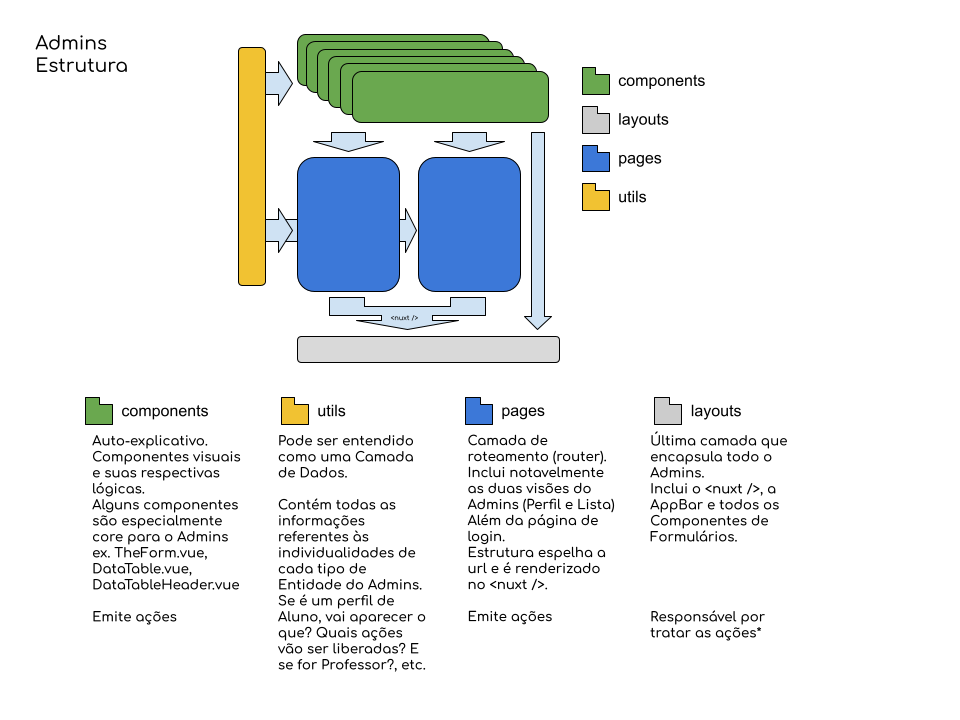
\includegraphics[width=1.0\linewidth]{Imagens/chap04/front-estrutura.png}
    \caption{Documentação criada para Jovens Gênios.}
    \label{fig:profile-exemple}
\end{figure}

\subsection{Uso da InstropectionQuery}

A IntrospectionQuery é uma requisição disponibilizada pela neo4j/graphql que pede ao servidor o schema de dados armazenado nele, além de quais são as consultas (queries) e mutações (mutations) permitidas pela API. Assim conseguimos não só conhecer todas as requisições possíveis, seus argumentos e tipos, como também todos os \textit{tipos} definidos nas definições de tipos e cada uma de suas propriedades. Utilizamos tais informações, por exemplo, quando abrimos um formulário de edição, utilizando a resposta para montar dinamicamente o formulário ou as tabelas nas quais os dados vão frequentar. Se acrescentarem mais uma propriedade na definição de tipos no backend, automaticamente o frontend vai mostrar um campo para esta, sem nenhum deploy ou alteração necessária.
(Preocupações de Segurança do instropection query)

Tal abordagem de construção dinâmica de formulários e perfis é interessante e foi utilizada durante alguns meses, porém percebemos que muitas vezes não queremos que o usuário desse gerenciador tenha acesso direto à edição de alguns dos atributos de alguns nós. Alguns atributos são pensados para serem populados automaticamente por outros fluxos e não esperado que editados manualmente, e outros simplesmente são dados utilizados “debaixo dos panos” - mostrar qualquer propriedade automaticamente no sistema ``Admins'' acabava confundindo os usuários.

Optamos então para uma abordagem híbrida, na qual recebemos no frontend quais são os atributos do \textit{tipo} referente na montagem dos formulários de criação e edição - porém os filtramos, mostrando apenas os que são editáveis, através de mapas em arquivos guardados no "utils". Esta abordagem híbrida também é utilizada nas colunas das tabelas das listas, e em quais as propriedades que aparecem no cabeçalho do perfil.

Abaixo um exemplo de um dos arquivos JSON do diretório "utils" que é usado para definir as propriedades à serem mostradas em cada cabeçalho de cada perfil, e como devem ser mostrados.
\begin{lstlisting}
{
  "Student": {
    "header": [
      "Id",
      "email",
      "schoolYear",
      "points",
      "keys",
      "trophies",
      "provider",
      "externalId"
    ],
    "chips": [],
    "rects": [
      {
        "prop": "questionsAnsweredCount",
        "extra": "Questoes Feitas",
        "color": "#5C9CE5"
      },
      {
        "prop": "correctQuestionsAnsweredCount",
        "extra": "Corretas",
        "color": "#5C9CE5"
      }
    ]
  },
...
\end{lstlisting}

o componente de busca e filtragem da página de listas também se beneficia do InstrospectionQuery, pois consegue, de forma automática listar todas as possibilidades de uma certa propriedade ENUM em um seletor. Sabendo qual o tipo de cada propriedade consegue colocae um input adequado para o usuário interagir.

\subsection{Formulário reutilizável}

\begin{lstlisting}
<v-form>
  <v-row no-gutters justify="end">
    <v-col cols="12" class="px-2">
      <v-text-field disabled label="Id" v-model="Id" outlined>
      </v-text-field>
    </v-col>
    
    <v-col
      cols="12"
      class="px-2"
      v-for="(property, i) in properties.strings"
      :key="i"
    >
      <v-row no-gutters>
        <v-col>
          <v-text-field
            :label="`${
              non_null[i] ? translate(i) + ' *' : translate(i)
            }`"
            v-model="property.value"
            :disabled="property.disableInput"
            outlined
          />
        </v-col>
        <v-col cols="11" v-if="i == 'avatarUrl'">
          <v-file-input
            @change="uploadImage(i, $event)"
            :label="`${
              non_null[i] ? translate(i) + ' *' : translate(i)
            }`"
            prepend-icon=""
            append-icon="$file"
            outlined
          >
          </v-file-input>
        </v-col>
      </v-row>
    </v-col>
    <v-col
      cols="6"
      class="px-2"
      v-for="(enumProperty, j) in properties.enums"
      :key="j"
    >
      <v-select
        :label="`${non_null[j] ? translate(j) + ' *' : translate(j)}`"
        :items="enumValues[j]"
        item-text="name"
        item-value="name"
        v-model="enumProperty.value"
        outlined
        @input="checkEnumChanged(enumProperty)"
      >
        <template slot="selection" slot-scope="{ item }">
          {{ translate(item.name) }}
        </template>
        <template slot="item" slot-scope="{ item }">
          {{ translate(item.name) }}
        </template>
      </v-select>
    </v-col>
    <v-col
      cols="6"
      class="px-2"
      v-for="(property, k) in properties.numerics"
      :key="k"
    >
      <v-text-field
        :label="`${non_null[k] ? translate(k) + ' *' : translate(k)}`"
        type="number"
        v-model="property.value"
        outlined
      />
    </v-col>
    <v-col
      cols="12"
      class="px-2"
      v-for="(property, w) in properties.dateTimes"
      :key="w"
    >
      <date-time-picker
        :label="`${non_null[w] ? translate(w) + ' *' : translate(w)}`"
        :datetime="property.value"
        @onChange="changedDateTime($event, w)"
      />
    </v-col>
    <v-col
      cols="5"
      v-if="
        isCreateTaskInSchoolClassProfile ||
        (classes.length > 1 && typename == 'Task')
      "
    >
      <v-switch
        class="mt-0"
        v-model="addAllStudentsFromSchoolClasses"
        label="Conectar com todos os alunos"
      ></v-switch>
    </v-col>

    <v-col cols="12" v-if="changedPassword">
      <v-text-field
        v-model="password"
        label="Nova Senha"
        outlined
      ></v-text-field>
    </v-col>
    
    <v-col
      cols="3"
      class="pb-2"
      v-for="(property, y) in properties.booleans"
      :key="y"
    >
      <v-switch
        class="mt-0"
        v-model="property.value"
        :label="`${non_null[y] ? translate(y) + ' *' : translate(y)}`"
      ></v-switch>
    </v-col>
  </v-row>
</v-form>
\end{lstlisting}

Além das propriedades editáveis do \textit{tipo}, que possuem um componente de interação específico dependendo de seu tipo. O sistema Admins possui também algumas ações e regras de negócios específicas em alguns formulários, que também são incluidas com a diretiva v-if em uma propriedade que define se tal ação ou regra de negócio específica deve estar ativa.

\begin{lstlisting}
    <v-col cols="12" v-if=" isCreateSchool">
      <courses-picker
        @changedCourses="changedCoursesSelected"
      ></courses-picker>
    </v-col>
    ...
    isCreateSchool() {
      return this.$route.params.type == "School" && this.add == true;
    }
\end{lstlisting}


\subsection{Ações}

As ações de manipulações de dados foram classificadas em três categorias:
\begin{itemize}
    \item Ações de Perfil - Em toda página de perfil de um nó, é possível abrir o formulário de ações diretas no nó dono. Inclue a deleção, edição de suas propriedades, e opcionalmente outras ações personalizadas
    \item Ações de Aba - Em cada aba dentro de um perfil, no cabeçalho de suas listas de elementos e com uma cor mais escura, existe botões de ações referentes à relações do nó dono com outros nós do \textit{tipo} referente à aba selecionada. Inclue a criação de um novo nó, já conectado ao dono, conectar o dono à um nó existente do \textit{tipo} da Aba, e opcionalmente outras ações personalizadas
    \item Ações de Elementos - Em cada aba dentro de um perfil, no cabeçalho de suas listas de elementos e com uma cor mais clara, é possível interagir com botões de ações referentes à elementos da lista selecionados. Inclue a edição do nó selecionado, e a desconexão dele(s) ào dono, além de opcionalmente outras ações personalizadas
\end{itemize}
Toda ação, independente da categoria, é propagada à camada Controle, carregando consigo um objeto com as informações que a definem. Nessa camada então, com acesso ao(s) \textit{tipo(s)} referente(s), seu(s) id(s), conseguimos escolher qual dos arquivos .gql que contém a requisição á ser enviada ao servidor deve ser utilizado na requisição.
\begin{figure}
    \centering
    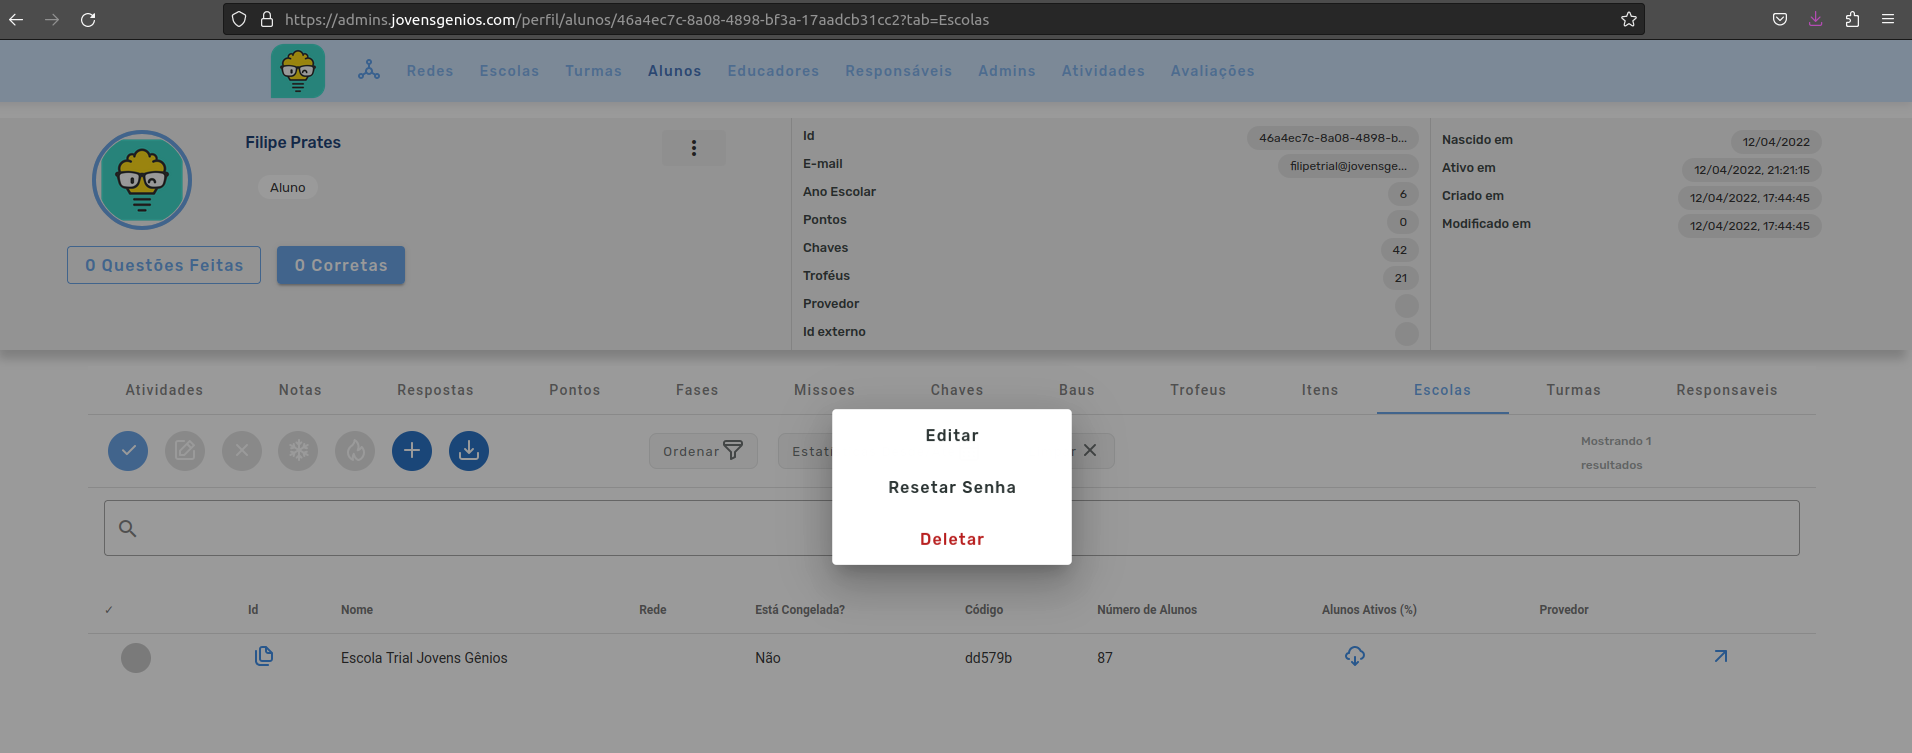
\includegraphics[width=1\linewidth]{Imagens/chap04/front-profile-actions.png}
    \caption{Interface das Ações de Perfil de um nó com \textit{tipo} Aluno}
    \label{fig:enter-label}
\end{figure}

\begin{figure}
    \centering
    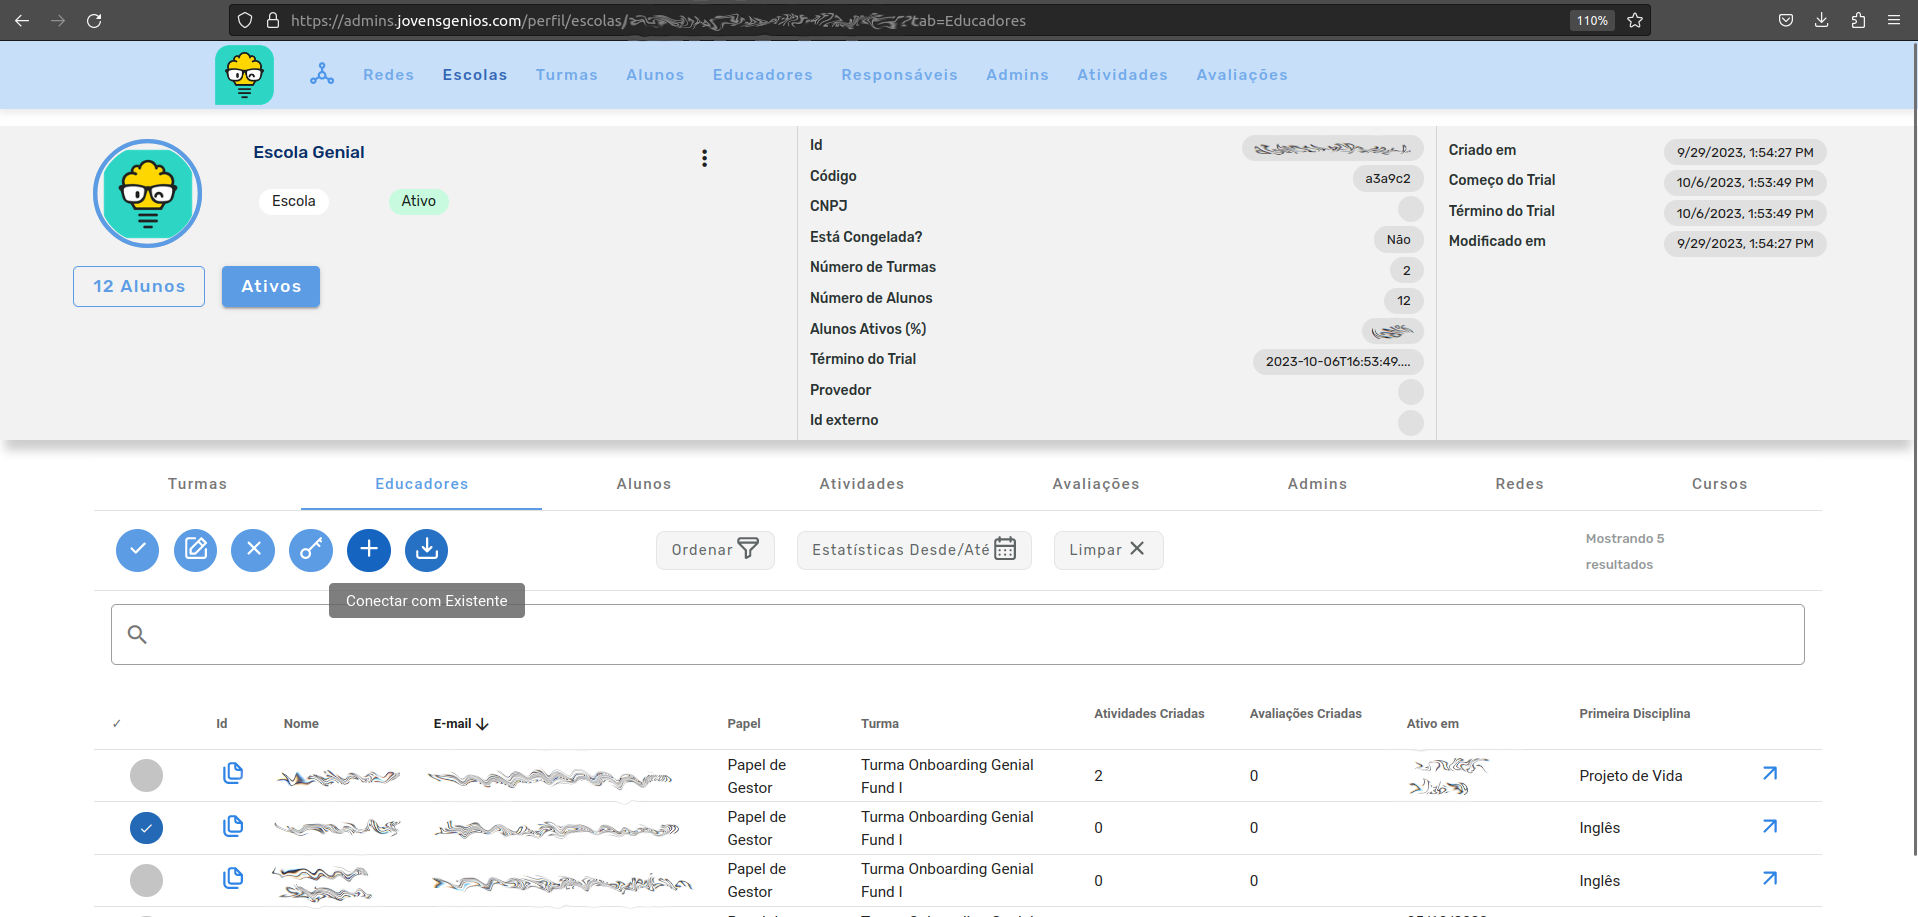
\includegraphics[width=1\linewidth]{Imagens/chap04/front-other-actions.png}
    \caption{Ações de Elementos e de Abas de um perfil do \textit{tipo} Escola, na Aba de relações com o \textit{tipo} Educadores.}
    \label{fig:enter-label}
\end{figure}


Abaixo um exemplo de função da camada de controle que lida com a ação de deletar múltiplos elementos selecionados de uma lista.

\begin{lstlisting}
async handleDelete(payload) {
  let type = "";
  for (let el of payload.elements) {
    if (confirm(`Certeza que quer deletar ${el.name}`)) {
        try {
          await this.$apollo.mutate({
            mutation: require(`@/graphql/${payload.type}/delete.gql`),
            variables: el,
          });
        } catch (e) {
          console.error(e);
          alert(e);
          return;
        }
      }
    }
  }
\end{lstlisting}

\section{Arquitetura do Servidor com endpoint GraphQL}

O frontend, entretando, não se comunica diretamente com o banco de dados, a interface se comunica com uma camada intermediária através de requisições em GraphQL, e esta camada intermediária gera a Cypher resultante que então é executado no banco de dados. Nesta seção descreveremos como funciona e a arquitetura escolhida para esta camada intermediária, o servidor que disponibiliza a endpoint em Graphql.

 \begin{figure}[H]

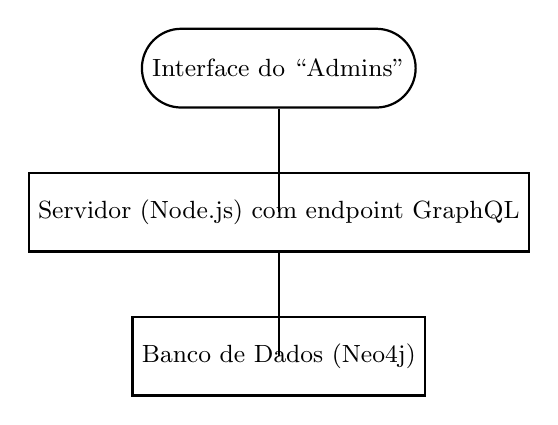
\begin{tikzpicture}[font=\small,thick]
 
% Start block
\node[draw,
    rounded rectangle,
    minimum width=2.5cm,
    minimum height=1cm] (block1) { Interface do ``Admins'' };
 
% Voltage and Current Measurement
\node[draw,
    below=0.8cm of block1,
    minimum width=2.5cm,
    minimum height=1cm
] (block2) { Servidor (Node.js) com endpoint GraphQL };
 
% Power and voltage variation
\node[draw,
    below=0.8cm of block2,
    minimum width=2.5cm,
    minimum height=1cm
] (block3) { Banco de Dados (Neo4j) };

\draw (block1) |- (block2);
\draw (block2) |- (block3);

\end{tikzpicture}
\caption{Fluxograma de comunicação entre partes do sistema }
\label{chap3:fluxograma}
\end{figure}

\subsection{Definições dos Tipos}

Uma das principais funções do servidor é a definição de cada \textit{tipo} existente no banco de dados. E nessa etapa, equivalente à definição das tabelas e campos num banco de dados SQL, que modelamos os dados do domínio e definimos cada \textit{tipo} de entidade que poderá ser manipulada através sistema gerenciador.

Como se tratam de muitos tipos diferentes, os separamos em diferentes arquivos para fim de organização, cada um com seu escopo. As definições de \textit{tipo} de cada arquivo respeitam um escopo definido, e possuem suas propriedades e tipos das propriedades, suas relações e tipos dos nós que são relacionados, além de definir aquelas Queries e Mutations que não são geradas automaticamente. Nestes arquivos, definimos também os tipos não nativos, como ENUMs específicos do escopo.

Os \textit{tipos} definidos geram as Labels que podem ser associadas aos nós do banco de dados.

Segue abaixo um exemplo simplificado de um arquivo de definição de tipos.
\begin{lstlisting}
"""
Battles types
"""
type Battle implements Context @node(labels: ["Battle", "Context"]) {
	id: ID @id
	name: String
	type: ContextType
	status: ContextStatus
	createdAt: DateTime! @timestamp(operations: [CREATE])
	updatedAt: DateTime! @timestamp(operations: [CREATE, UPDATE])
	assignedContext: [AssignedContext!]!
		@relationship(type: "OF_CONTEXT", direction: IN)
	studentAnswers: [StudentAnswer]
		@cypher(
			statement: """
			MATCH (this)<-[:OF_CONTEXT]-(:AssignedContext)<-[:OF_ASSIGNED_CONTEXT]-(sa:StudentAnswer) return distinct sa
			"""
		)
	topic: Topic @relationship(type: "SELECTED_IN_BATTLE", direction: OUT)
	task: Task @relationship(type: "BATTLE_IN_TASK_CONTEXT", direction: OUT)
	fromOrigin: BattleOrigin #TODO: Improve the property
	students: [AssignedContext]
		@cypher(
			statement: """
			MATCH (this)<-[:OF_CONTEXT]-(ac:AssignedContext)-[:ASSIGNED_TO]->(s:Student) return distinct ac
			"""
		)
	startsAt: DateTime
	endsAt: DateTime
	knowledgeArea: KnowledgeArea
		@relationship(type: "IN_KNOWLEDGE_AREA", direction: OUT)
}

enum StudentBattleStatus {
	NotStarted
	InProgress
	Finished
	Refused
}

type Query {
	botQuestionAnswerFraction(
		studentProgressInPlanet: Float
		questionDifficulty: Float
	): Float
}

type Mutation {
	mergeStudentsBattle(
		studentsIds: [ID!]
		battleId: ID!
		type: ContextType
	): [ID]
	setBattleResult(battleId: ID!): String
	deleteBattle(battleId: ID!): ID
	setChampionshipBattleResults(championshipId: ID!): String
}
\end{lstlisting}

\subsection{Mesclador de Definições de Tipos}
A biblioteca Neo4j/GraphQL espera apenas um arquivo de definição de tipos, então precisamos juntar todos eles utilizando expressões regulares e os padrões de cada arquivo de definição de tipo.

\begin{lstlisting}
const fs = require("fs");
const path = require("path");

let typeDefs = "";
let mutations = "";
let queries = "";
let subscriptions = "";
const dirname = path.join(__dirname, "./types/");

export const mergeTypeDefs = () => {
	const filenames = fs.readdirSync(dirname);

	filenames.forEach((filename) => {
		let content = fs.readFileSync(dirname + filename, "utf-8");

		concatMutations(content);
		concatQueries(content);
		concatSubscriptions(content);

		content = removeMutationsQueriesAndSubscriptions(content);
		typeDefs += content;
	});

	typeDefs += mergeMutationsQueriesAndSubscriptions(typeDefs);

	return typeDefs;
};

const concatMutations = (typeDef) => {
	const re = /(?<=Mutation\s*\{)(.*?[\s\S]*?)(?=\n\}\n|\r\n\}\r\n)/g;
	const mutationsInTypeDef = typeDef.match(re);

	if (mutationsInTypeDef && mutationsInTypeDef.length > 0) {
		mutations = mutations.concat(...mutationsInTypeDef);
	}
};

const concatQueries = (typeDef) => {
	const re = /(?<=Query\s*\{)(.*?[\s\S]*?)(?=\n\}\n|\r\n\}\r\n)/g;
	const queriesInTypeDef = typeDef.match(re);

	if (queriesInTypeDef && queriesInTypeDef.length > 0) {
		queries = queries.concat(...queriesInTypeDef);
	}
};

const concatSubscriptions = (typeDef) => {
	const re = /(?<=Subscription\s*\{)(.*?[\s\S]*?)(?=\n\}\n|\n\}\n|\r\n\}\r\n)/g;
	const subscriptionsInTypeDef = typeDef.match(re);

	if (subscriptionsInTypeDef && subscriptionsInTypeDef.length > 0) {
		subscriptions = subscriptions.concat(...subscriptionsInTypeDef);
	}
};

const removeMutationsQueriesAndSubscriptions = (typeDef) => {
	const reMutations = /type\s*Mutation\s*\{(.*?[\s\S]*?)(\n\}\n|\r\n\}\r\n)/g;
	const reQueries = /type\s*Query\s*\{(.*?[\s\S]*?)(\n\}\n|\r\n\}\r\n)/g;
	const reSubscriptions = /type\s*Subscription\s*\{(.*?[\s\S]*?)(\n\}\n|\r\n\}\r\n)/g;

	let newTypeDef = typeDef.replaceAll(reMutations, "");
	newTypeDef = newTypeDef.replaceAll(reQueries, "");
	newTypeDef = newTypeDef.replaceAll(reSubscriptions, "");
	return newTypeDef;
};

const mergeMutationsQueriesAndSubscriptions = (typeDef) => {
	if (mutations.length > 0) {
		typeDef += `\r\n\r\ntype Mutation {\r\n${mutations}\r\n}`;
	}
	if (queries.length > 0) {
		typeDef += `\r\n\r\ntype Query {\r\n${queries}\r\n}`;
	}
	if (subscriptions.length > 0) {
		typeDef += `\r\n\r\ntype Subscription {\r\n${subscriptions}\r\n}`;
	}

	return typeDef;
};
\end{lstlisting}

\subsection{Os resolvers}

\subsection{Geração do Schema para o banco de dados}

 Utilizamos a bibliotecas do driver da Neo4j para conectar ao banco, autenticando com usuário e senha.
 
 \begin{lstlisting}
import neo4j from "neo4j-driver";

const driver = neo4j.driver(
	process.env.NEO4J_URI || "bolt://localhost:7687",
	neo4j.auth.basic(
		process.env.NEO4J_USER || "neo4j",
		process.env.NEO4J_PASSWORD || "neo4j"
	),
	{
		maxConnectionLifetime: 8 * 60 * 1000,
		maxConnectionPoolSize: 50,
		connectionAcquisitionTimeout: 2 * 60 * 1000,
		disableLosslessIntegers: true,
	}
);
\end{lstlisting}

Então importamos os nossos resolvers e definições de tipos, e configuramos os plugins utilizados, como o Neo4jGraphQLAuthJWTPlugin, que permite a autenticação das requisições através de uma JWToken no campo de "Authorization" no header de cada requisição GraphQL.

 O Schema é então gerado instanciando um novo objeto Neo4jGraphQL() (da @neo4j/graphql), que recebe como argumentos o driver conectado ao banco de dados, as definições de \textit{tipos} mescladas, os resolvers e eventuais plugins.

\begin{lstlisting}
import { Neo4jGraphQL } from "@neo4j/graphql";
import { Neo4jGraphQLAuthJWTPlugin } from "@neo4j/graphql-plugin-auth";
const typeDefs = mergeTypeDefs();
async function initializeNeo4jGraphQL() {
	const neo4jGraphQL = new Neo4jGraphQL({
		driver,
		typeDefs: gql`
			${typeDefs}
		`,
		resolvers,
		plugins: {
			auth: new Neo4jGraphQLAuthJWTPlugin({
				secret: process.env.JWT_SECRET,
				algorithms: ["HS256"],
				credentialsRequired: false,
			}),
			config: {
				enableDebug: process.env.NODE_APP_ENV === "staging",
			},
		},
	});
	return await neo4jGraphQL.getSchema();
}
\end{lstlisting}

Em seguida o Apollo Server é inicializado com este Schema e o servidor express o publica nas portas definidas, aguardando as requisições.

\begin{lstlisting}
import { expressMiddleware } from "@apollo/server/express4";
    const app = express();
    app.use(cors());
    app.use(json({ limit: "20mb" }));
    app.use(express.urlencoded({ limit: "20mb", extended: true }));
    
	const apolloServer = new ApolloServer({
		schema: schema,
		introspection: true,
		playground: process.env.NODE_APP_ENV !== "production",
		plugins: [
			ApolloServerPluginLandingPageGraphQLPlayground(),
			{
				async serverWillStart() {
					return Promise.resolve({
						async drainServer() {
							await serverCleanup.dispose();
						},
					});
				},
			},
		],
	});

	app.use(
		path,
		expressMiddleware(apolloServer, {
			context: ({ req }) => ({
				driver,
				neo4jDatabase: process.env.NEO4J_DATABASE,
				req
			}),
		})
	);
\end{lstlisting}


\begin{lstlisting}
const port = process.env.GRAPHQL_SERVER_PORT || 4001;
const path = process.env.GRAPHQL_SERVER_PATH || "/graphql";
const host = process.env.GRAPHQL_SERVER_HOST || "0.0.0.0";

const httpServer = createServer(app);
const wsServer = new WebSocketServer({
	server: httpServer,
	path: path,
});

httpServer.listen({ host, port, path }, () => {
		console.log(`GraphQL server ready at http://${host}:${port}${path}`);
		console.log(`WS Subscriptions ready at ws://${host}:${port}${path}`);
});


\end{lstlisting}




    \chapter{Sistema em Operação}
\label{chap5}


\section{Jovens Gênios Provedor de Conteúdo LTDA}

A Jovens Gênios surgiu em 2016 com Fernando Costa, aluno da Escola de Química da UFRJ e apaixonado por Educação, procurando soluções de ensino extracurriculares engajantes para seus irmãos mais novos. Seguindo uma lógica "efetual"[1] 
Effectuation: Elements of Entrepreneurial Expertise
, não satisfeito com as soluções existentes,desenvolveu plataformas de apoio ao processo de ensino-aprendizagem embrionárias, tendo os irmãos como primeiros usuários.
Junto com o antigo colega Bernard Caffé, que compartilhava a paixão por educação, tendo experiência como professor e com o estudo de Metodologias Ativas de aprendizado, fundaram a empresa Jovens Gênios, tendo escolas de bairro como seus primeiros clientes.

A experiência foi bem sucedida, sendo hoje, seis anos depois, utilizada por centenas de milhares de usuários/alunos de todo o Brasil, os quais registraram através das plataformas Jovens Gênios centenas de milhões de respostas em questões.

\section{Modelagem do Domínio}

O caso de uso da Jovens Gênios inclui nós das estruturas escolares (Redes de ensino, Escolas, Turmas, Alunos, Professores, Gestores), nós do conteúdo gerado pela empresa (Questões, Resumos, Tópicos, Cursos, Disciplinas), nós das atividades que acontecem nas plataformas (Desafios, Tarefas, Provas Somativas, Provas Diagnósticas, Batalhas, Campeonatos, Aulas Invertidas), e, principalmente, os nós referentes às respostas dos alunos, que conectam o aluno à questão e ao contexto da atividade que levou o aluno àquela questão.

A estrutura em árvore dos tópicos e da estrutura escolar, assim como a facilidade de realizar a manutenção e desenvolver novas funcionalidades com as ferramentas disponíveis, foram os fatores determinantes para a escolha de um banco em grafo.

\section{Solução para Supernós}

Supernós são nós que possuem muitos relacionamentos relativos ao resto da rede. Tais nós podem surgir de maneira natural dada uma rede densamente conectada, porém podem causar problemas para o sistema gerenciador do banco de dados do Neo4j.

O driver disponível da Neo4j, apesar de conter e permitir múltiplos acessos de leitura simultâneos ao banco de dados, bloqueia os nós referentes quando executa uma escrita, como por exemplo uma conexão de um nó com outro.
Quando múltiplos usuários simultâneos realizam ações repetitivas que geram nós que se conectam sempre ao mesmo nó, temos impacto no tempo de resposta senão falha crítica do banco de dados.

Encontramos tais problemas pela primeira vez em um Desafio aberto à todos os alunos da plataforma por um tempo limitado. Nesse período, todas as respostas à questões geradas na plataforma eram conectadas a um mesmo desafio. A solução encontrada para diminuir o acesso mútiplo de escrita ao mesmo nó foi introduzir um nó intermediário entre o aluno e um Desafio no momento que este é liberado à ele, e as respostas (e qualquer outra da interação entre o Desafio e o Aluno) são conectadas nesse nó intermediário, ao invés de diretamente no Desafio em si.

    \begin{figure}[H]
        \centering
        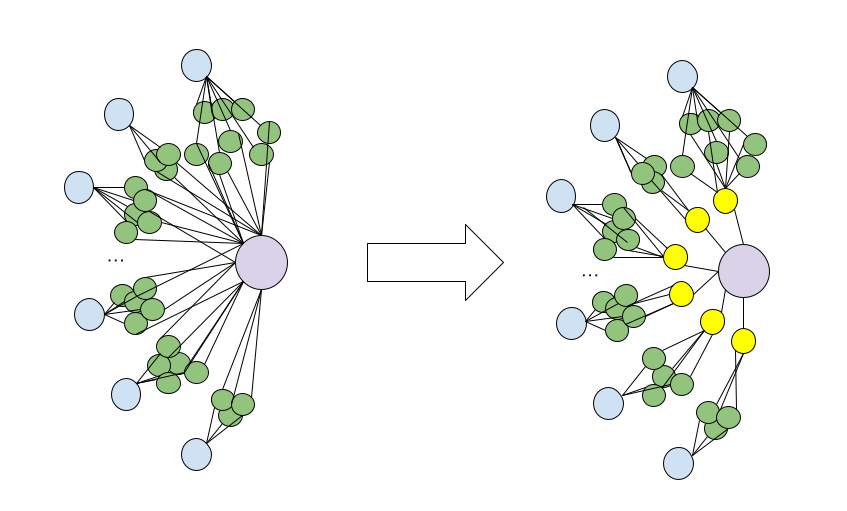
\includegraphics[width=1.0\linewidth]{Imagens/chap05/AssignedContext.png}
        \caption{\(n\) Alunos, \(k = [k_1, k_2, k_3, .., k_n]\) respostas e um Desafio conectados diretamente, e através de nós intermediários}
        \label{fig:profile-exemple}
    \end{figure}
Dessa forma, cada aluno (nó que gera os outros nós) tem um nó para si, e as operações de escrita bloqueantes antes executadas no único nó central agora são distribuídas entre os nós intermediários.

\(n:k:1\) onde o nó central recebe \(\sum_{i=1}^n k_i\) requisições de conexões, vira \(n:k:n:1\), onde nenhum nó recebe mais de do \(k_{max}\) conexões.

Tal modelagem impactou o sistema "Admins", ficando menos intuitivo a navegação entre o perfil do Aluno e suas Atividades (não só desafios, qualquer atividade que poderia ter uma quantidade significativa de alunos simultâneos online). Decidimos que o ideal era esconder o nó intermediário da navegação, e o clique em um elemento do nó intermediário na tabela redireciona o usuário diretamente ao perfil da atividade (ou aluno) do outro lado. As respostas sendo resolvidas por um cypher personalizado ao schema pelos dois lados.

\section{Papeis dos Usuários do sistema ``Admins''}

Os seguintes perfis de colaboradores são usuários do sistema ``Admins'' na Jovens Gênios:

\begin{itemize}
    \item Educacional (Responsáveis pelo contato direto com as escolas e definição das turmas)
    \item Suporte (Contato online com alunos e professores para esclarecer dúvidas, mapear e resolver eventuais problemas)
    \item Controle De Qualidade (Auxílio para setup de testes e entendimento do comportamentos das plataformas em diferentes casos)
    \item Desenvolvedores (Visualizar estado do banco de dados e realizar eventuais manipulações)
\end{itemize}

    \chapter{Conclusões}
\label{chap6}
 \section{Trabalhos Futuros}
 
Generalização para qualquer endpoint Graphql - backend blind
  \backmatter
  %\nocite{*}
  \bibliographystyle{coppe-unsrt}
  \bibliography{thesis}
  \appendix
  \chapter{Código Fonte Aberto}
\label{apendice}

Tabela é muito chato fazer, vou deixar alguns exemplo para seguir, mas eu gosto bastante de utilizar esse site aqui para gerar as tabelasa de forma mais fácil: https://www.tablesgenerator.com/

%%%%%%%%%%%%%%%%%%%%%%%%%%%%%%%%%%%%%%%%%%%%%%%%%%%%%%
%%%%%%  COLOCAR TABELAS DE SEÇÕES DE CHOQUE  %%%%%%%%%
%%%%%%%%%%%%%%%%%%%%%%%%%%%%%%%%%%%%%%%%%%%%%%%%%%%%%%

\begin{table}[H]
\centering
\caption{Parâmetros de geração dos produtos de fissão (\cite{belo2022}).} \label{tab:generationPF} \vspace{0.5cm}
\begin{tabular}{llcccc}
\hline
\textbf{$i$} & \textbf{Actinídeos} & \multicolumn{1}{l}{\textbf{$\gamma_{ij}$}} & \multicolumn{1}{l}{\textbf{}} & \multicolumn{1}{l}{\textbf{}} & \multicolumn{1}{l}{\textbf{}} \\ \hline
\textbf{}    & \textbf{}           & \textbf{$j = 16$}                          & \textbf{$j = 18$}             & \textbf{$j = 19$}             & \textbf{$j = 20$}             \\
\textbf{}    & \textbf{}           & \textbf{$^{149}$Pm}                      & \textbf{$^{135}$I}          & \textbf{$^{135}$Xe}         & \textbf{LFP}                \\ \hline
1            & $^{234}$U           & 0,0107                                     & 0,0630                        & 0,0024                        & 1,0                           \\
2            & $^{235}$U           & 0,0107                                     & 0,0630                        & 0,0024                        & 1,0                           \\
3            & $^{236}$U           & 0,0107                                     & 0,0630                        & 0,0024                        & 1,0                           \\
4            & $^{237}$Np          & 0,0107                                     & 0,0630                        & 0,0024                        & 1,0                           \\
5            & $^{238}$U           & 0,0161                                     & 0,0683                        & 0,0003                        & 1,0                           \\
6            & $^{238}$Pu          & 0,0124                                     & 0,0645                        & 0,0115                        & 1,0                           \\
7            & $^{239}$Np          & 0,0000                                     & 0,0000                        & 0,0000                        & 0,0                           \\
8            & $^{239}$Pu          & 0,0124                                     & 0,0645                        & 0,0115                        & 1,0                           \\
9            & $^{240}$Pu          & 0,0124                                     & 0,0645                        & 0,0115                        & 1,0                           \\
10           & $^{241}$Pu          & 0,0152                                     & 0,0707                        & 0,0023                        & 1,0                           \\
11           & $^{241}$Am          & 0,0152                                     & 0,0707                        & 0,0023                        & 1,0                           \\
12           & $^{242}$Pu          & 0,0152                                     & 0,0707                        & 0,0023                        & 1,0                           \\
13           & $^{242}$Cm          & 0,0152                                     & 0,0707                        & 0,0023                        & 1,0                           \\
14           & $^{243}$Am          & 0,0152                                     & 0,0707                        & 0,0023                        & 1,0                           \\
15           & $^{244}$Cm          & 0,0152                                     & 0,0707                        & 0,0023                        & 1,0                           \\ \hline
\end{tabular}
\end{table}



\begin{table}[H]
\centering
\caption{Seções de choque microscópicas para o decaimento do tipo $n2n$ do $^{238}$U (\cite{belo2022}).} \label{tab:n2nU238} \vspace{0.5cm}
\begin{tabular}{lc}
\hline 
\textbf{\begin{tabular}[l]{@{}l@{}}Região\\ {}\end{tabular}} & \begin{tabular}[c]{@{}c@{}}$\sigma_{n2n,g}^{U238}$\\ {[barn]}\end{tabular}   \\ \hline 
FA01                                                                    & 6,17E-03                                                                   \\  
FA02                                                                    & 6,17E-03                                                                  \\ 
FA03                                                                    & 6,17E-03                                                                   \\ 
FA04                                                                    & 6,17E-03                                                                   \\ \hline 
\end{tabular}
\end{table}


\definecolor{lightgray}{rgb}{.9,.9,.9}
\definecolor{darkgray}{rgb}{.4,.4,.4}
\definecolor{purple}{rgb}{0.65, 0.12, 0.82}

\end{document}
